
%%%%%%%%%%%%%%%%%%%%%%%%%%%%%%%%%%%%%%%%%%%%%%%%%%%%%%%%%%%%%%%%%%%%%%%%%%%%%%
% Copyright (c) 2003-2015 by The University of Queensland
% http://www.uq.edu.au
%
% Primary Business: Queensland, Australia
% Licensed under the Open Software License version 3.0
% http://www.opensource.org/licenses/osl-3.0.php
%
% Development until 2012 by Earth Systems Science Computational Center (ESSCC)
% Development 2012-2013 by School of Earth Sciences
% Development from 2014 by Centre for Geoscience Computing (GeoComp)
%
%%%%%%%%%%%%%%%%%%%%%%%%%%%%%%%%%%%%%%%%%%%%%%%%%%%%%%%%%%%%%%%%%%%%%%%%%%%%%%

\section{Slip on a Fault}\label{Slip CHAP}
\begin{figure}[ht]
\centerline{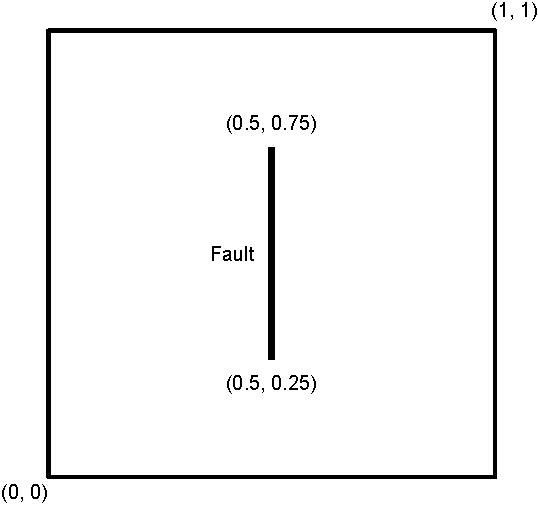
\includegraphics{Slip1}}
\caption{Domain $\Omega=[0,1]^2$ with a vertical fault of length $0.5$.}
\label{fig:slip.1}
\end{figure}
%
In this example we illustrate how to calculate the stress distribution around
a fault\index{fault} in the Earth's crust caused by a slip\index{slip} through
an earthquake.

To simplify the presentation we assume a simple domain $\Omega=[0,1]^2$ with
a vertical fault in its center as illustrated in \fig{fig:slip.1}.
We assume that the slip distribution $s_{i}$ on the fault is known.
We want to calculate the distribution of the displacements $u_{i}$\index{displacement}
and stress $\sigma_{ij}$\index{stress} in the domain.
Further, we assume an isotropic, linear elastic material model of the form
\begin{eqnarray} \label{Slip  stress}
\sigma_{ij} & = & \lambda u_{k,k} \delta_{ij} + \mu ( u_{i,j} + u_{j,i})
\end{eqnarray}
where $\lambda$ and $\mu$ are the Lam\'e coefficients\index{Lam\'e coefficients}
and $\delta_{ij}$ denotes the Kronecker symbol\index{Kronecker symbol}.
On the boundary the normal stress is given by
\begin{eqnarray} \label{Slip natural fault}
\sigma_{ij}n_{j}=0
\end{eqnarray}
and normal displacements are set to zero:
\begin{eqnarray} \label{Slip constraint}
u_{i}n_{i} =0
\end{eqnarray}
The stress needs to fulfill the momentum equation\index{momentum equation}
\begin{eqnarray}\label{Slip general problem}
- \sigma_{ij,j}=0
\end{eqnarray}
This problem is very similar to the elastic deformation problem presented in \Sec{ELASTIC CHAP}.
However, we need to address an additional challenge: the displacement
$u_{i}$ is in fact discontinuous across the fault, but we are in the
lucky situation that we know the jump of the displacements across the fault.
This is in fact the given slip $s_{i}$.
So we can split the total distribution $u_{i}$ into a component
$v_{i}$ which is continuous across the fault and the known slip $s_{i}$
\begin{eqnarray}\label{Slip Split}
u_{i} = v_{i} + \frac{1}{2} s^{\pm}_{i}
\end{eqnarray}
where $s^{\pm}=s$ when right of the fault and $s^{\pm}=-s$ when left of the fault.
We assume that $s^{\pm}=0$ when sufficiently away from the fault.

We insert this into the stress definition in \eqn{Slip stress}
\begin{eqnarray} \label{Slip stress split}
\sigma_{ij} & = &
\sigma^c_{ij} +
\frac{1}{2} \sigma^s_{ij}
\end{eqnarray}
 with
\begin{eqnarray} \label{Slip stress split 1}
\sigma^c_{ij} = \lambda v_{k,k} \delta_{ij} + \mu ( v_{i,j} + v_{j,i})
\end{eqnarray}
and
\begin{eqnarray} \label{Slip stress split 2}
\sigma^s_{ij} = \lambda s^{\pm}_{k,k} \delta_{ij} + \mu ( s^{\pm}_{i,j} + s^{\pm}_{j,i}).
\end{eqnarray}
In fact, $\sigma^s_{ij}$ defines a stress jump across the fault.
An easy way to construct this function is to use a function $\chi$ which is
$1$ on the right and $-1$ on the left side from the fault.
One can then set
\begin{eqnarray} \label{Slip  stress split 23 }
\sigma^s_{ij} = \chi \cdot  ( \lambda s_{k,k} \delta_{ij} + \mu ( s_{i,j} + s_{j,i}) )
\end{eqnarray}
assuming that $s$ is extended by zero away from the fault.
After inserting \eqn{Slip stress split} into (\ref{Slip general problem}) we
get the differential equation\index{momentum equation}
\begin{eqnarray}\label{Slip general problem 2 }
- \sigma^c_{ij,j}=\frac{1}{2} \sigma^s_{ij,j}
\end{eqnarray}
Together with the definition (\ref{Slip stress split 1}) we have a
differential equation for the continuous function $v_i$.
Notice that the boundary condition (\ref{Slip constraint}) and (\ref{Slip natural fault})
transfer to $v_i$ and $\sigma^c_{ij}$ as $s$ is zero away from the fault.
In \Sec{ELASTIC CHAP} we have discussed how this problem is solved using
the \LinearPDE class. We refer to this section for further details.

To define the fault we use the \class{FaultSystem} class introduced in \Sec{Fault System}.
The following statements define a fault system \var{fs} and add the fault \var{1} to the system:
\begin{python}
  fs=FaultSystem(dim=2)
  fs.addFault(fs.addFault(V0=[0.5,0.25], strikes=90*DEG, ls=0.5, tag=1)
\end{python}
The fault added starts at point $(0.5,0.25)$ has length $0.5$ and points north.
The main purpose of the \class{FaultSystem} class is to define a
parameterization of the fault using a local coordinate system.
One can inquire the class to get the range used to parameterize a fault.
\begin{python}
  p0,p1 = fs.getW0Range(tag=1)
\end{python}
Typically \var{p0} is equal to zero while \var{p1} is equal to the length of the fault.
The parameterization is given as a mapping from a set of local coordinates
onto a parameter range (in our case the range \var{p0} to \var{p1}).
For instance, to map the entire domain \var{mydomain} onto the fault one can
use
\begin{python}
  x = mydomain.getX()
  p,m = fs.getParametrization(x, tag=1)
\end{python}
Of course there is the problem that not all locations are on the fault.
For those locations which are on the fault \var{m} is set to 1, otherwise 0 is used.
So on return the values of \var{p} define the value of the fault parameterization
(typically the distance from the starting point of the fault along the fault)
where \var{m} is positive.
On all other locations the value of \var{p} is undefined.
Now \var{p} can be used to define a slip distribution on the fault via
\begin{python}
  s = m*(p-p0)*(p1-p)/((p1-p0)/2)**2*slip_max*[0.,1.]
\end{python}
Notice the factor \var{m} which ensures that \var{s} is zero away from the fault.
It is important that the slip is zero at the ends of the faults.

We can now put all components together to get the script:
\begin{python}
  from esys.escript import *
  from esys.escript.linearPDEs import LinearPDE
  from esys.escript.models import FaultSystem
  from esys.finley import Rectangle
  from esys.weipa import saveVTK
  from esys.escript.unitsSI import DEG

  #... set some parameters ...
  lam=1.
  mu=1
  slip_max=1.
  mydomain = Rectangle(l0=1.,l1=1.,n0=16, n1=16)  # n1 needs to be a multiple of 4!
  # .. create the fault system
  fs=FaultSystem(dim=2)
  fs.addFault(V0=[0.5,0.25], strikes=90*DEG, ls=0.5, tag=1)
  # ... create a slip distribution on the fault
  p, m=fs.getParametrization(mydomain.getX(), tag=1)
  p0,p1= fs.getW0Range(tag=1)
  s=m*(p-p0)*(p1-p)/((p1-p0)/2)**2*slip_max*[0.,1.]
  # ... calculate stress according to slip:
  D=symmetric(grad(s))
  chi, d=fs.getSideAndDistance(D.getFunctionSpace().getX(), tag=1)
  sigma_s=(mu*D+lam*trace(D)*kronecker(mydomain))*chi
  #... open symmetric PDE ...
  mypde=LinearPDE(mydomain)
  mypde.setSymmetryOn()
  #... set coefficients ...
  C=Tensor4(0., Function(mydomain))
  for i in range(mydomain.getDim()):
    for j in range(mydomain.getDim()):
       C[i,i,j,j]+=lam
       C[j,i,j,i]+=mu
       C[j,i,i,j]+=mu
  # ... fix displacement in normal direction
  x=mydomain.getX()
  msk=whereZero(x[0])*[1.,0.] + whereZero(x[0]-1.)*[1.,0.] \
     +whereZero(x[1])*[0.,1.] + whereZero(x[1]-1.)*[0.,1.]
  mypde.setValue(A=C, X=-0.5*sigma_s, q=msk)
  #... solve pde ...
  mypde.getSolverOptions().setVerbosityOn()
  v=mypde.getSolution()
  # .. write the displacement to file:
  D=symmetric(grad(v))
  sigma=(mu*D+lam*trace(D)*kronecker(mydomain))+0.5*sigma_s
  saveVTK("slip.vtu", disp=v+0.5*chi*s, stress=sigma)
\end{python}
The script creates the file \file{slip.vtu} which contains the total
displacements and stress.
These values are stored as cell-centered data.
%
\begin{figure} [ht]
\centerline{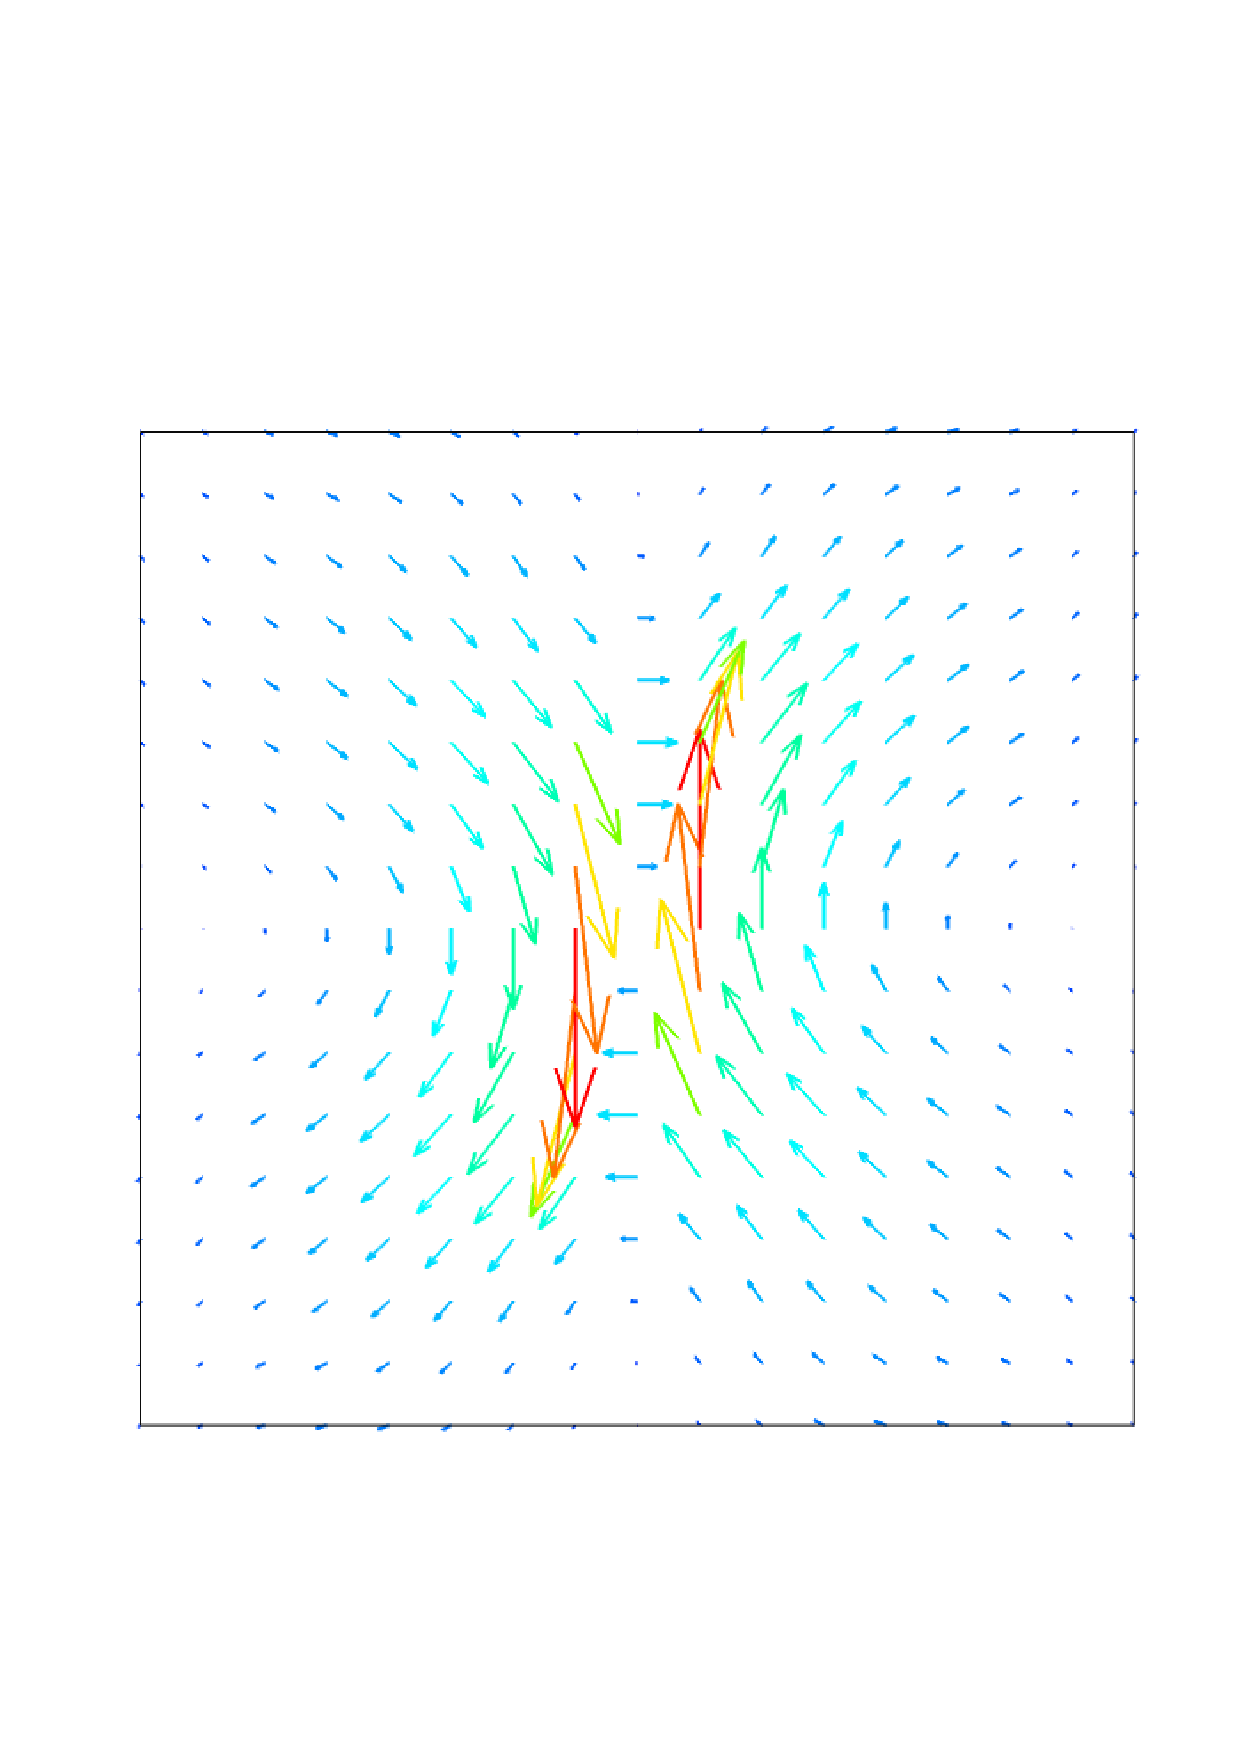
\includegraphics[width=\figwidth]{Slip2}}
\caption{Total Displacement after the slip event}
\label{fig:slip.2}
\end{figure}
%
See \fig{fig:slip.2} for a visualization of the result.

